\subsection{You Only Look Once}

Der Algorithmus \textit{You Only Look Once} (YOLO) ist ein weiterer Objekterkennungsalgorithmus und betrachtet statt separaten Bildregionen das komplette Bild. Er benutzt nur ein neuronales Netz, um Bounding Boxen und Wahrscheinlichkeiten für bestimmte Klassen vorherzusagen.

Hierzu wird ein $S \times S$ Gitter über das Bild gelegt. Für jedes Feld im Gitter werden $B$ Bounding Boxen erzeugt. Jede Box besitzt neben den zum Gitterfeld relativen Positionswerten einen Wert, der die Vorhersage der jeweiligen Klasse und die Präzision der Box repräsentiert. Dieser Wert wird als \textit{confidence score} bezeichnet und wird durch die Multiplikation der Wahrscheinlichkeit für eine Klasse mit der \textit{IoU}, also die Präzision der berechneten Box im Verhältnis zu der Box aus den vortrainierten Testdaten festgelegt \cite{JosephRedmon.2016}.

Aus der Menge an Bounding Boxen werden schließlich mit Hilfe eines festgelegten Schwellwertes die Boxen mit lokalisierten Objekten bestimmt (siehe Abbildung \ref{yolo_model}).

\begin{figure}[ht]
	\begin{center}
		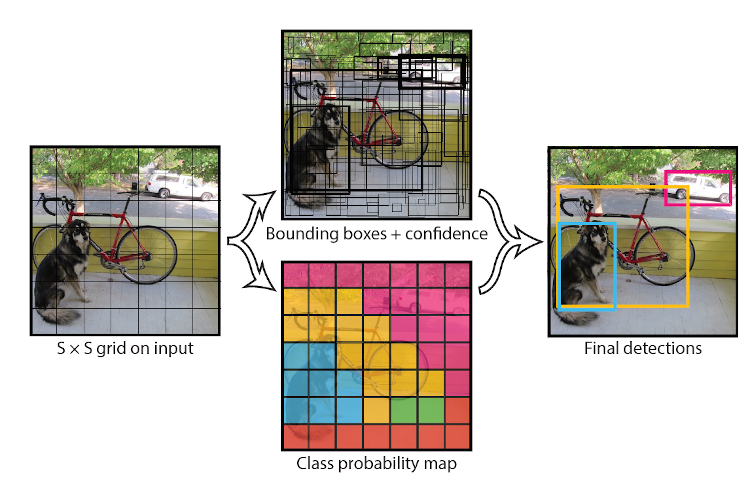
\includegraphics[width=15cm]{Bilder/yolo_model.png} 
		\caption{Vereinfachte Darstellung der Objekterkennung mit dem YOLO Algorithmus \cite{JosephRedmon.2016}}
		\label{yolo_model}
	\end{center}
\end{figure}

\newpage

Die vorhergesagten Werte werden in einem $S \times S \times (B * 5 + C)$ Tensor kodiert, wobei $S$ und $B$ wie zuvor beschrieben durch das Gitter und die Bounding Boxen festgelegt sind und $C$ die Anzahl der Klassen definiert. Abbildung \ref{yolo_architecture} zeigt den Aufbau des CNN von \textit{YOLO} für die Detektion. Es besteht aus 24 Convolutional Layern gefolgt von 2 Fully-connected Layern. Für die Genauigkeit bei der Detektion wird die Auflösung des Bildes verdoppelt \cite{JosephRedmon.2016}. 

Im Modell in Abbildung \ref{yolo_architecture} wird folglich ein Bild mit einer Auflösung von $224 \times 224$ verwendet und die vorhergesagten Werte im $7 \times 7 \times 30$ Tensor ausgegeben. 

\begin{figure}[ht]
	\begin{center}
		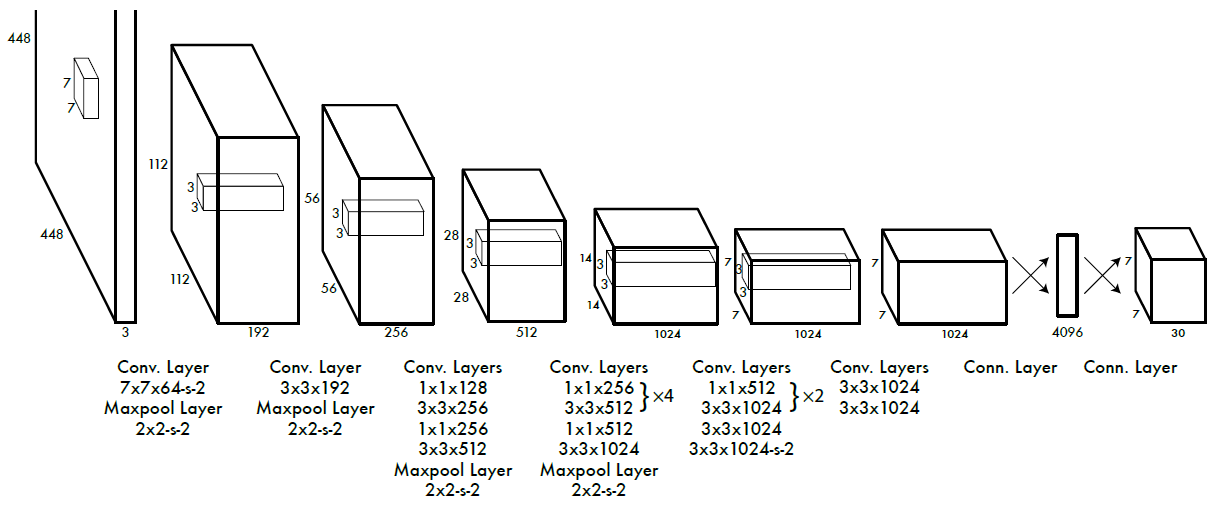
\includegraphics[width=15cm]{Bilder/yolo_architecture.png} 
		\caption{\textit{YOLO} Architektur \cite{JosephRedmon.2016}}
		\label{yolo_architecture}
	\end{center}
\end{figure}






